\section{Concepción y Diseño}\label{section:design}

\begin{figure}
    \centering
    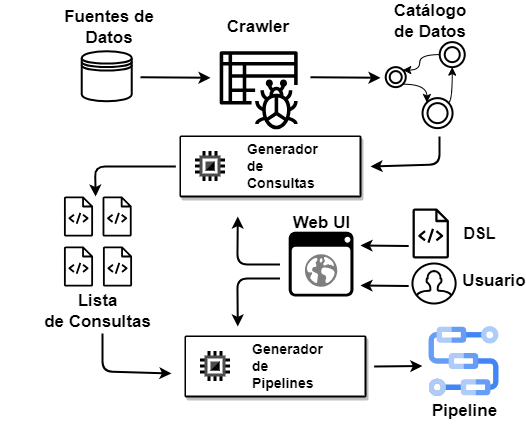
\includegraphics[width=0.60\textwidth]{Graphics/arch.drawio.png}
    \caption{Arquitectura del prototipo de AutoETL}
    \label{fig:arquitectura}
    \end{figure}

AutoETL se concibe como una herramienta para ser utilizada por los desarrolladores de almacenes de datos 
con el objetivo de aliviar la carga de trabajo en la implementaci\'on de los procesos de población de las 
estructuras analíticas. Como se observa en la Figura \ref{fig:arquitectura} los componentes de la aplicaci\'on 
est\'an dispuestos de forma secuencial para representar el flujo de trabajo de la herramienta.

\begin{itemize}
    \item El primer elemento de la arquitectura propuesta son las \textbf{Fuentes de Datos}. En esta primera concepción del 
        prototipo solo se pueden manejar bases de datos relacionales y una fuente de datos a la vez.
    \item La tarea del \textbf{Crawler} es explorar las fuentes de datos para recopilar información relevante sobre su estructura, 
        con el fin de crear el \textbf{Catálogo de Datos} a partir de dicha información.
    \item El \textbf{Catálogo de Datos} es una estructura que almacena metadatos sobre las fuentes de datos, los cuales son 
        utilizados en el proceso de la generaci\'on de consultas.
    \item Los usuarios interactúan con la herramienta a través de una interfaz web. Mediante esta interfaz, especifican el modelo 
        analítico a poblar, establecen conexiones con las fuentes de datos, consultan metadatos, configuran opciones necesarias 
        para el proceso de generación de consultas y del pipeline, y finalmente ejecutan el pipeline generado. El escenario analítico 
        es especificado mediante un script del lenguaje de dominio espec\'ifico, dicho script debe ser programado por el usuario en 
        un editor de c\'odigo de su preferencia.
    \item El \textbf{Generador de Consultas} es el encargado de tomar la información proveniente del Catálogo de Datos, de la especificaci\'on
        del escenario analítico y de las configuraciones del usuario, para generar una lista de consultas que creen y pueblen el escenario 
        analítico en cuesti\'on.
    \item El \textbf{Generador de Pipelines} tiene la tarea de crear el pipeline para la población y creaci\'on del escenario analítico, partiendo 
        de la lista de consultas generadas por le generador de consultas y de las especificaciones del usuario para la creaci\'on del pipeline.
    \item Por \'ultimo, el pipeline es una estructura en la que est\'a correctamente especificado el orden de ejecuci\'on de las consultas, 
        el m\'etodo de carga y captura de los datos para la población, y la frecuencia con que se ejecutar\'a el pipeline.
\end{itemize}

En las secciones a continuación se expone de forma general el funcionamiento de
los distintos módulos del sistema y las principales consideraciones tomadas durante
su diseño.

\subsection{Crawler}

Este componente tiene la tarea de explorar las fuentes de datos para recopilar metadatos \'utiles para el proceso de generaci\'on
de consultas. Los metadatos extra\'idos son los nombres de las tablas de la base de datos fuente, por cada tabla se obtienen sus 
atributos, por cada atributo su tipo y si son llaves primarias. Adem\'as por cada tabla se obtienen los atributos que son llaves 
for\'aneas y por cada una, se extrae la tabla a la que referencian y el atributo referenciado. Con esta información se construye 
el catálogo de datos.

\subsection{Catálogo de Datos}

Una vez que los metadatos de la fuente de datos son recopilados por el Crawler se pasa a construir el Catálogo de Datos. Este componente 
es un multigrafo dirigido donde los nodos representan las tablas de la base de datos fuente y entre dos nodos $v$, $w$ 
del catálogo existe un arco $<v,w>$ por cada llave for\'anea en $v$ que referencie a un atributo de $w$. Cada nodo (tabla) guarda 
los nombres de los atributos de la tabla que representa, sus tipos y si son llaves primarias, for\'aneas o ambas. Cada arco $<v,w>$ 
guarda una tupla donde el la primera posici\'on se encuentra el nombre del atributo de $v$ que es llave for\'anea y en la segunda 
posici\'on el nombre del atributo de $w$ referenciado. N\'otese que la direcci\'on de un arco representa el sentido de la 
referencia de la llave for\'anea a la que representa.

\subsection{Lenguaje de Dominio Especifico}

Como parte de los objetivos de la presente investigaci\'on est\'a la concepción y diseño de un lenguaje de dominio 
espec\'ifico para la definici\'on de escenarios analíticos. El objetivo del lenguaje es servir de v\'inculo 
entre el modelo relacional de la fuente de datos y el modelo dimensional del escenario analítico. El lenguaje 
brinda recursos sintácticos para la especificaci\'on de tablas de dimensiones y tablas de hechos, las cuales 
en su conjunto constituyen la definicion de un esquema estrella.

La definici\'on de atributos en las tablas de hechos o de dimensi\'on constituye la base del v\'inculo entre 
el modelo relacional de la fuente y el modelo dimensional del escenario analítico. La definición de un atributo 
implica detallar la procedencia y los valores que lo constituirán, es decir, la tabla de donde se extraerán los 
valores (el 'dónde'), 
así como identificar el atributo concreto dentro de esa tabla cuyos valores se usarán para completar el atributo 
que estamos definiendo (el 'con qué'). Este proceso garantiza que cada atributo se defina de manera clara y que 
se alimente correctamente con los datos pertinentes. De esta forma se entrelazan la definici\'on relacional 
de la fuente de datos con el modelo dimensional del esquema estrella. A continuación se presenta la gramática 
libre del contexto que da definición al DSL propuesto. Las palabras en may\'uscula indican no terminales y 
las palabras en min\'uscula indican terminales.

\begin{lstlisting}[caption={Gram\'atica libre del contexto del lenguaje de dominio espec\'ifico}]
    S' -> Dimensional_Model
    Dimensional_Model -> List_Dimensional_Tables
    List_Dimensional_Tables -> Dimensional_Table
                    | List_Dimensional_Tables Dimensional_Table

    Dimensional_Table -> dimension ID { List_Attr_Def }
                       | fact ID { List_Attr_Def }

    List_Attr_Def -> Attr_Def
                   | List_Attr_Def Attr_Def

    Attr_Def -> Attr_Expression Type Alias Level

    Attr_Expression -> T X
    X -> + T X | - T X | empty
    T -> F Y
    Y -> * F Y | / F Y | empty
    F -> Attr | number | (Attr_Expression)

    Attr -> Table : ID Modifier
          | Table : Func ( ID )
          | Table : sum ( ID )
          | Table : avg ( ID )
          | Table : count ( ID )
          | Table : max ( ID )
          | Table : min ( ID )

    Table -> ID | self

    Func -> weekday | monthstr

    Alias -> as ID | empty

    Level -> number | empty

    Type -> int | str | date | datetime | serial | float | numeric 
          | empty

    Modifier -> pk | fk to ID . ID | empty
\end{lstlisting}

%TODO: Agregar definicion de multigrafo en el marco teorico

Tal y como dicta la gramática, un modelo dimensional (\textbf{Dimensional\_Model}), 
en el contexto del DSL, est\'a compuesto por una lista de tablas 
dimensionales. 

Una lista de tablas dimensionales (\textbf{List\_Dimensional\_Tables}) est\'a compuesta por al menos 
una definici\'on de tabla dimensional 
(\textbf{Dimensional\_Table}), aunque es cierto que un esquema estrella no tiene sentido si tiene una sola tabla 
de dimensi\'on o una sola tabla de hechos, expresar la restricci\'on en la gramática de que una lista de 
tablas dimensionales debe tener al menos una tabla de dimensi\'on y una tabla de hechos es un proceso 
engorroso que puede atentar contra la legibilidad de la gramática, por tanto se decide dejar dicha 
comprobaci\'on para los chequeos sem\'anticos que se le efect\'uan a las instancias del lenguaje provistas 
por el usuario, luego de ser parseadas. 

Luego, la 
definición de una tabla dimensional (\textbf{Dimensional\_Table}) consta de la palabra clave dimension o fact, 
en caso de querer definir una dimension o una tabla de hechos respectivamente, un nombre para dicha tabla 
(\textbf{ID}), llaves con funci\'on delimitadora (\textbf{\{\}}) y dentro de estas una lista de definiciones de atributos
(\textbf{List\_Attr\_Def}). 

Una lista de definiciones de atributos est\'a compuesta por al menos una definición de atributo (\textbf{Attr\_Def}). 
La definición de un atributo consta de una expresión de atributos (\textbf{Attr\_Expression}), un tipo para el atributo 
definido, dicho tipo (\textbf{Type}) puede especificarse o no, un alias (\textbf{Alias}) que en caso de no ser vacío ser\'a el nombre del 
atributo en el esquema estrella y un nivel (\textbf{Level}) que es un entero que especifica la profundidad 
del atributo definido en la jerarqu\'ia de la dimensi\'on. Una expresión de atributos (\textbf{Attr\_Expression}) no es m\'as que 
un recurso gramatical para expresar que una definición de atributo puede ser tanto un solo atributo (\textbf{Attr})
como una expresi\'on aritm\'etica en la que pueden participar atributos y n\'umeros. 

Un atributo (\textbf{Attr}) es la representaci\'on en el DSL de un atributo de la fuente de datos. Est\'a compuesto, 
fundamentalmente, 
por el nombre de la tabla de la fuente de datos (\textbf{Table}), dos puntos y el nombre del atributo de dicha tabla 
de donde se obtendr\'an los valores (\textbf{ID}). Adem\'as puede contener especificaciones de modificadores (\textbf{Modifier}), 
los cuales pueden ser especificaciones de llave primaria o llave for\'anea. En esta primera versi\'on del 
DSL un atributo puede ser llave primaria o llave for\'anea, pero no los dos a la vez. Tambi\'en, a los valores
extra\'idos del atributo con nombre (\textbf{ID}) y tabla (\textbf{Table}) se le puede aplicar funciones o agregaciones. Las 
funciones de agregaci\'on implementadas son suma (\textbf{sum}), promedio (\textbf{avg}), conteo (\textbf{count}), m\'aximo (\textbf{max}) y 
m\'inimo (\textbf{min}). Las funciones implementadas en esta primera versi\'on son \textbf{weekday}, la cual a partir de 
una fecha devuelve el d\'ia de la semana, y \textbf{monthstr} que devuelve el nombre del mes de una fecha pasada 
como argumento. La palabra reservada self solo se debe usar para declarar la tabla en la definición de atributos 
que sean llaves primarias autogeneradas para las tablas de hechos.

Los tipos manejados por el lenguaje son gen\'ericos y facilmente mapeables con los tipos de los sistemas de 
gesti\'on de bases de datos relacionales m\'as usados. El tipo \textbf{int} engloba a los n\'umeros enteros. 
Al tipo \textbf{str} pertenecen las cadenas de texto. Los tipos \textbf{date} y \textbf{datetime} agrupan a las fechas y a las fechas con 
hora respectivamente. El tipo \textbf{serial} se usa para las llaves primarias autogeneradas. El tipo \textbf{float} 
representa a los n\'umeros con coma flotante. Finalmente, al tipo \textbf{numeric} pertenecen todos los valores numéricos.

En caso de que una definición de un atributo solo contenga un atributo de una tabla de la fuente no es necesario 
especificar el tipo, pues el sistema autom\'aticamente asignar\'a el tipo del atributo fuente al tipo del 
atributo que est\'a siendo definido. Sin embargo si se define un atributo compuesto, es decir, un atributo que 
en su definición participe m\'as de un atributo de la fuente, es necesario especificar el tipo pues el sistema 
no es capaz de inferirlo.

Para especificar una llave for\'anea se deben escribir las palabras reservadas \textbf{fk} y \textbf{to} y luego especificar 
el nombre de una tabla del esquema estrella, un punto y el atributo referenciado.

Para asignar un alias a un atributo definido para una tabla del modelo dimensional se utiliza la 
palabra reservada \textbf{as} seguida del nombre del atributo.


\subsection{Generador de Consultas}

Este componente es el m\'as importante y el de mayor responsabilidad dentro de la arquitectura. Es el encargado 
de generar el c\'odigo SQL necesario para la creaci\'on y población del escenario analítico. Las consultas generadas 
se dividen en dos grupos: el grupo de creaci\'on de tablas y el grupo de selecci\'on de valores. El primer grupo 
son las consultas de creaci\'on de cada una de las tablas del esquema estrella. El segundo grupo son las  consultas 
que seleccionan los atributos necesarios para la población de una tabla del esquema estrella. 

Las dimensiones, generalmente, est\'an formadas por atributos de distintas tablas de las fuentes de datos, por 
ejemplo, una dimension que expresa la ubicaci\'on geogr\'afica se forma por la uni\'on de las tablas municipio, 
provincia y pa\'is. En las bases de datos relacionales con un diseño correcto, es usual encontrarse estos 
tres conjuntos de entidades separados en tablas normalizadas, enlazadas mediante llaves for\'aneas, con el objetivo 
de evitar duplicaci\'on de datos y anomal\'ias en la inserci\'on, modificaci\'on y eliminaci\'on. Por tanto, el 
proceso de selecci\'on de datos para la población de la dimensi\'on ubicaci\'on geogr\'afica pasa por unir las 
tablas municipio, provincia y pa\'is, para poder extraer los datos desde una única tabla, es 
decir, denormalizar la jerarqu\'ia impuesta por el proceso de normalizaci\'on sobre las tablas municipio, provincia
y pa\'is. La uni\'on de esas tablas se logra mediante la aplicaci\'on del join pertienente.

En las tabla de hechos sucede algo similar, puede que los valores de un hecho se encuentren en una 
sola tabla o que en su calculo intervengan atributos de múltiples tablas de la fuente, en ese caso 
el procedimiento es el mismo que con el ejemplo de la dimensi\'on ubicaci\'on geogr\'afica. Es necesario 
unir todas las tablas que intervengan en el c\'alculo del hecho en cuesti\'on mediante joins.

Luego una parte fundamental del proceso de población de un escenario anal\'itico es la implementaci\'on 
de estos joins. Precisamente, el Generador de Consultas implementado es el encargado, entre otras cosas, de inferir los 
joins necesarios en la construcci\'on de las consultas de selecci\'on de valores, que son las encargadas de la 
extracci\'on de los datos de las tablas fuente que poblaran las tablas del escenario anal\'itico.

En otras ocasiones, se ha enfrentado el problema de la inferencia de consultas utilizando representaciones
de bases de datos en forma de grafos y lenguajes 
de dominio espec\'ifico. Entre estos trabajo se pueden mencionar aquellos que definen lenguajes de consulta 
conceptuales (Conceptual Query Languajes, CQL) que tratan de ocultar la dificultad de un esquema de bases de 
datos relacionando conceptos familiares con el usuario y entidades de la base de datos. Con este enfoque 
podemos citar los trabajos \cite{owei2001enriching} el cual propone
un algoritmo basado en caminos m\'inimos para encontrar el camino m\'as corto de joins que una conceptos 
especificados, dando como resultado una sola interpretaci\'on de la consulta, lo cual no es factible 
puesto que lo ideal es analizar todas las posibles interpretaciones para una consulta y escoger la 
que sem\'anticamente responda a las necesidades del usuario. Otro enfoque para abordar el problema 
es mediante algoritmo de busqueda de palabras clave (Keyword Search Algorithms, KSA), especificamente  
aquellos que orientan la b\'usqueda sobre grafos. N\'otese que teniendo un conjunto de palabras clave 
a buscar (atributos que unir en una sola tabla), la respuesta es un sub\'arbol del grafo de b\'usqueda 
el cual para toda palabra buscada exista un nodo que la contenga. Los trabajos 
\cite{kimelfeld2006finding,hristidis2003efficient,he2007blinks} exponen algoritmos eficientes para 
encontrar, dado k, las k mejores interpretaciones, es decir, los k mejores sub\'arboles que dan respuesta 
a la consulta, m\'as su dependencia al par\'ametro k para explorar todas las posibles interpretaciones 
hizo que el autor se decantara por la propuesta de \cite{mason2005autojoin} para la resoluci\'on 
del problema de la inferencia de los joins planteado en los objetivos de la presente investigaci\'on.

El enfoque seleccionado parte de un grafo de join, que no es m\'as que un grafo con las mismas caracter\'isticas 
del Cat\'alogo de Datos solo que empaca la información de los m\'ultiples arcos que pueden existir entre 
dos nodos del cat\'alogo en un \'unico arco y adem\'as, añade un arco $<v, w>$ si el nodo $v$ contiene un subconjunto 
de atributos contenidos en $w$ tal que todos los miembros de dicho subconjunto sean llaves for\'aneas en $v$
y en $w$ sean llaves primarias. N\'otese que estos subconjuntos de atributos cumplen con las restricciones 
de una llave for\'anea aunque dicha relaci\'on entre ambas tablas no est\'a explicita en la base de datos, 
y por tanto constituyen un join v\'alido.

Dado un conjunto de atributos fuente que conforman una dimensi\'on o una tabla de hechos, el join necesario 
para unir estos atributos en una tabla \'unica es un sub\'arbol del grafo de join. Pero, este join no tiene 
porque ser \'unico, pueden existir otros sub\'arboles que tambi\'en constituyan joins v\'alidos para lograr 
la uni\'on de los atributos. 

Explorar todos los posibles sub\'arboles durante una consulta sobre el grafo de join mediante 
recorridos sucecivos es ineficiente. Para resolver este problema \cite{mason2005autojoin} propone 
generar, a partir del grafo de join, sub\'arboles maximales. Cada sub\'arbol maximal, al tener un juego 
de arcos diferentes, aporta potencialmente un join distinto. En el resto del documento estos sub\'arboles 
maximales ser\'an referidos como \'arboles de join. Una consulta sobre estos \'arboles no es m\'as que 
un conjunto de nodos (tablas) a unir. Una respuesta a una consulta sobre un \'arbol de join es un sub\'arbol 
del mismo cuyos nodos hojas sean los nodos de la consulta, y esto constituye una interpretaci\'on 
de la consulta para dicho  \'arbol de join.

Propuestas anteriores a \cite{mason2005autojoin} proponen para computar los \'arboles de join hallar 
el subgrafo alcanzable desde un nodo y a este sub\'arbol calcularle todos los posibles \'arboles de 
expansi\'on, los cuales constituyen los \'arboles de join. Repitiendo este proceso para cada nodo se lograba 
calcular el conjunto de \'arboles de join, 
pero estos enfoques daban como resultado \'arboles de join duplicados y sobre todo 
es un algoritmo ineficiente y no computable para grafos de gran tamaño.

El planteamiento de \cite{mason2005autojoin} introduce mejoras a este algoritmo. Establece que un \'arbol 
de join debe ser maximal, de no serlo, es posible que exista un \'arbol de join m\'as extenso que lo contenga. 
Tal \'arbol de join ampliado sería capaz de proporcionar, no solo 
los joins posibilitados por el \'arbol de join inferior en tamaño sino también adicionales, debido a que engloba 
un mayor número de nodos y, por ende, tiene la capacidad de brindar joins para consultas inaccesibles a su 
contraparte más limitada. Siguiendo esta idea, se propone solo computar el grafo alcanzable 
a nodos del grafo de join que tengan grado interior (indegree) igual a cero o que est\'en en una 
componente fuertemente conexa en la que no existan arcos incidentes externos a la misma. 
Los \'arboles de join emanados de estos nodos raíz son inherentemente maximales, ya que la naturaleza de su raíz, 
implica que no hay otro subárbol que pueda subsumir los generados por dicha raíz.

Ahora, como el conjunto de \'arboles de join depende solamente del esquema de base de datos y no de las consultas
este puede ser precomputado, trasladando fuera del tiempo de consulta la computaci\'on m\'as costosa. La cantidad
de \'arboles de join depende \'unicamente de la ambiguedad inherente del esquema de base de datos. Una esquema 
de base de datos no ambiguo resultar\'a en un u\'nico \'arbol de join y, por ende, en una \'unica interpretaci\'on 
para cada consulta. Las ambiguedades m\'as comunes se materializan en el grafo de join como nodos con m\'as de 
un arco incidente a \'el y como componentes fuertemente conexas.

\subsubsection{Fase de precomputaci\'on}

La fase de precomputaci\'on se encarga de dado un grafo de join, calcular los \'arboles de join. Como se expuso 
anteriormente se identifican las posibles ra\'ices, se halla el grafo alcanzable para cada una de las ra\'ices. 
Por cada grafo alcanzable se computan sus \'arboles de expansi\'on. El conjunto de todos los \'arboles en 
expansi\'on calculados es el conjunto de \'arboles de join del grafo de join dado. Los \'arboles de join 
son almacenados y recuperados cuando se nececite responder una consulta. El algoritmo utilizado para calcular 
los \'arboles de expansi\'on (spanning trees) de los grafos alcanzable es el propuesto por Harold N. Gabow y 
Eugene W. Myers en 1978 \cite{gabow1978finding}. El listado de c\'odigo \ref{precom} muestra el pseudoc\'odigo 
del proceso de precomputaci\'on.

\begin{lstlisting}[label={precom}, caption={Pseudoc\'odigo del proceso de precomputaci\'on}]
    precomputation (JoinGraph dg)
    {
        allSCC = strongly connected components of dg
        rGraphs = empty
        for each scc in allSCC
            if (size scc == 1 and node has no in-edges)
                rGraphs = rGraphs + findReachable(n);
            else
                for each node n in scc
                    if (n has no in-edges from outside scc)
                        rGraphs = rGraphs + findReachable(n);
        joinTrees = empty
        for each reachable graph g in rGraphs
            joinTrees = joinTrees + findSpanningTrees(g)
        return joinTrees
    }
\end{lstlisting}

La demostraci\'on de que este algoritmo produce todos \'arboles de join se puede encontrar en 
\cite{mason2005autojoin}. Con respecto a la complejidad temporal, el algoritmo de Harold N. Gabow y 
Eugene W. Myers tiene complejidad temporal $O(|V| + |E| + |E|N)$ donde $|V|, |E|, N$ son la cardinalidad 
del conjunto de v\'ertices, la cardinalidad del conjunto de arcos y la cantidad de \'arboles de expansi\'on. 
Esta complejidad temporal, dentro del ciclo, es la que domina en el algoritmo. El n\'umero de \'arboles de 
expansi\'on de un grafo dirigido puede ser exponencial en el caso peor, caso en que el grafo de join sea 
completo, por tanto la complejidad temporal de este algoritmo en el caso peor es exponencial. Sin embargo, 
el caso peor, un esquema de bases de datos completamente conectado, no es com\'un y la mayor\'ia de esquemas 
poseen un n\'umero razonable de \'arboles de join. Adem\'as, la precomputaci\'on solo se realiza una vez, 
cuando se descubre el esquema de la base de datos y solo se vuelve a realizar la precomputaci\'on si dicho 
esquema sufre cambios en su definición.

\subsubsection{Fase de consulta}

Para dar respuesta a las consultas, es decir, el devolver un conjunto de joins que constituyen 
interpretaciones de la consulta, el procedimiento es identificar los \'arboles de join que 
contengan todos los nodos (tablas) de la consulta. Luego por cada \'arbol de join identificado 
se busca el ancestro com\'un m\'as bajo (lowest common acestor, LCA) de este conjunto de nodos. 
El sub\'arbol del \'arbol de join que da respuesta a la consulta y que constituye un join v\'alido 
para la uni\'on de las tablas, se forma mediante la uni\'on de los caminos desde 
el LCA hasta los nodos requeridos. El listado de c\'odigo \ref{querytime} muestra el pseudoc\'odigo 
del algoritmo que computa la lista de joins asociados a una consulta.

\begin{lstlisting}[label={querytime}, caption={Pseudoc\'odigo del algoritmo de inferencia de joins}]
    get_joins (List_of_JoinTrees jts, List_of_Query_Tables query)
    {
        valid_join_trees = identify_join_trees(jts, query)
        all_joins = empty
        for each join_tree in valid_join_trees
            lca = lowest_common_acestor(join_tree, query)
            join = reconstruc_sub_tree(join_tree, lca, query)
            all_joins = all_joins + join

        return all_joins
    }
\end{lstlisting}

Basado en toda la teor\'ia expuesta anteriormente, resulta bastante f\'acil corroborar la correctitud del 
algoritmo. La construcci\'on de los \'arboles de joins garantiza que el sub\'arbol reconstruido mediante el 
LSA constituye un join v\'alido y el algoritmo devuelve todos los joins posibles para una consulta pues 
precisamente el conjunto de \'arboles de join representan correctamente todas las posibles formas de 
unir mediante joins las tablas de la base de datos.

Para el an\'alisis de complejidad temporal se denota como $Q$ a la cantidad de tablas que contiene la consulta, 
$N$ a la cantidad de \'arboles de joins, $|V|$ a la cantidad de nodos del \'arbol de join m\'as extenso y $|E|$
a su cantidad de arcos. 

Calcular la interseccion de dos conjunto con $s$ y $t$ elementos respectivamente tiene 
complejidad temporal $O(s + t)$ si se utilizan conjuntos hash. Se añaden los $s$ elementos al conjunto hash en $O(1)$
y luego por cada uno de los $t$ elementos se pregunta si est\'an en el conjunto hash en $O(1)$, los elementos 
que se confirmen que est\'an en el conjunto hash conforman el conjunto intersección. Luego de estas aclaraciones 
se puede pasar al an\'alisis de la complejidad temporal del algoritmo.

Para identificar que \'arboles de join contienen todos los nodos de la consulta se puede implementar un índice 
inverso donde cada tabla (nodo) se enlaza a todos los árboles de join que contienen 
este nodo. La intersección de los conjuntos de árboles de join da como resultado todos los árboles de join 
que contienen todos los nodos especificados. Este procedimiento puede realizarse en $O(QN)$. 

El LCA se computa hallando la intersecci\'on entre todos los acestros de las tablas de consulta y luego 
seleccionando el m\'as bajo en altura como LCA. Para una tabla (nodo) de la consulta hallar sus ancestros 
tiene complejidad $O(|V| + |E|)$ empleando DFS tomando el reverso de los arcos, este proceso se realiza $Q$ veces
para computar los ancestros de cada uno de los $Q$ nodos. 
Hallar la intersección 
entre todos los ancestros de los nodos requeridos se realiza tomando un conjunto de ancestros 
como conjunto inicial y hallando la intersección de este conjunto con el resto de conjuntos de ancestros, 
resultando al final en el conjunto de ancestros comunes, este procedimiento tiene complejidad temporal 
$O(Q(|V| + |V|)) = O(Q(2|V|)) = O(Q|V|)$ asumiendo el caso peor que es que todos los conjuntos de acestros 
tengan cardinalidad $|V|$. Luego de tener los ancestros comunes se identifica el que contenga menor altura 
en $O(|V|)$ resultando que el computo del LCA para un conjnto de nodos de tamaño $Q$ es $O(Q(|V| + |E|))$

Reconstruir el sub\'arbol que se forma mediante la uni\'on de los caminos desde el LCA hasta los nodos 
de la consulta tiene complejidad temporal $O(|V| + |E|)$. Añadir elementos a una lista tiene complejidad 
$O(1)$ u $O(n)$ en dependencia de la implementaci\'on de lista que se utilice, siendo $n$ la cantidad 
de elementos de la lista, por simplicidad del an\'alisis se toma como $O(1)$.

Finalmente, el algoritmo realiza por cada \'arbol de join una b\'usqueda de LCA, una reconstrucci\'on 
del sub\'arbol para ese LCA y se añade el sub\'arbol a una lista. Resultando en una complejidad 
temporal de $O(NQ(|V| + |E|))$.


\subsubsection{Generaci\'on de c\'odigo}

Este componente también tiene la tarea de generar el c\'odigo SQL para la creaci\'on de las 
tablas del esquema estrella en el almac\'en de datos de destino y para la selecci\'on de 
los datos que alimentan el almac\'en desde la fuente. Para lograrlo este cometido se apoya 
del algoritmo de inferencia de joins y de las especificaciones del escenario anal\'itico 
mediante el lenguaje de dominio espec\'ifico. Por tanto, para inferir las consultas para 
la población y creaci\'on de un escenario anal\'itico es necesario que el desarrollador y 
usuario de la herramienta proporcione un script del DSL con la definición del escenario 
a poblar. Por cada tabla del esquema estrella se genera una consulta de creaci\'on y una 
consulta de selecci\'on.

Para construir la consulta de creaci\'on de una tabla del esquema estrella basta con recorrer 
la lista definiciones de atributos que expone el script para dicha tabla y agregar a la consulta 
su nombre, su tipo y su modificador. 
El nombre lo aporta el alias en el caso de atributos compuestos o en caso de ser un solo atributo 
se mantiene el nombre que posee en la fuente de datos de no tener un alias especificado. Luego se 
añaden las restricciones de llaves primarias y for\'aneas. Por \'ultimo, si se trata de una tabla 
de hechos se añade una restricci\'on de unicidad a la combinaci\'on de llaves for\'aneas a las 
dimensiones.

Para construir las consultas de selecci\'on de una tabla del esquema estrella se recorre la 
lista definiciones de atributos que expone el script para dicha tabla y se recolectan las 
tablas que intervienen en la definición de los atributos y los nombres de los atributos requeridos.
Se conforma una consulta con las tablas especificadas y se llama al algoritmo \textbf{get\_joins} 
pasando como argumentos la consulta y la lista de \'arboles de joins precomputados para el esquema 
de base de datos de la fuente, obteniendo as\'i una lista de posibles joins para unir todas las 
tablas que intervienen en la consulta.

En esta primera propuesta de la herramienta, el sistema no es capaz de inferir cu\'al es el join 
m\'as adecuado seg\'un las necesidades del usuario, dado que puede haber varios joins que resulten 
en la uni\'on de las tablas especificadas pero la sem\'antica del resultado no tiene por qu\'e ser 
la misma. Por tanto, luego de obtener la lista de joins el usuario debe seleccionar el que responda 
a sus intereses.

Luego de tener el join seleccionado, se pasa a construir la consulta. En la parte de la cl\'ausula 
\textbf{SELECT} se añaden todos los nombres de los atributos recolectados y en la secci\'on de la cl\'ausula 
\textbf{FROM} se coloca el join seleccionado. Si existen atributos resultado de agregaciones se añade 
la cl\'ausula \textbf{GROUP BY} con todos los atributos que intervienen en el select a los que no 
se les aplique una funci\'on de agregaci\'on.


\subsection{Generador de pipelines}

Luego de generar las consultas de creaci\'on y de selecci\'on, el usuario debe especificar 
mediante la interfaz gr\'afica el \'orden de ejecuci\'on de las consultas generadas, 
el tipo de extracci\'on de datos de la fuente que utilizar\'a el pipeline, el tipo de carga 
en el sistema de destino y la frecuencia con que se ejecutar\'a. Con esta información y las 
consultas generadas se conforma un pipeline. 

Las consultas de creaci\'on son mandadas a ejecutar en el sistema que albergar\'a el almac\'en de 
datos. Las consultas de selecci\'on son enviadas para su ejecuci\'on en el sistema fuente y el resultado 
es recepcionado por la herramienta implementada de acuerdo al tipo de extracci\'on seleccionado por el usuario. 
Luego se genera una consulta de inserci\'on para estos 
datos y por \'ultimo se ejecutan de acuerdo al tipo de carga especificado.
